\chapter{Unsupervised Approach}


The problem with supervised approaches is that they require that each class of interest is represented in the training dataset. However, with real human falls the variability of the environmental conditions and of the subjects makes difficult or impossible to collect a sufficient number of examples that allow the algorithm to generalize well on unseen conditions \cite{Noury2007}. Unsupervised approaches tackle the problem as a novelty detection task \cite{markou2003novelty1,markou2003novelty2}, i.e., by learning a normality model from data not related to human falls.


da qui in poi si usa solo il FAS poerchè è stato appurato che è migliore dei microfoi aerei

\section{Novelty detection algorithm for human fall detection based on One-Class Support Vector Machine}
\label{sec:ocsvm_approach}

The approach proposed in this section is based on a One-Class Support Vector Machine (OCSVM) \cite{scholkopf2000} to obtain an unsupervised framework for Fall Detection.
The acoustic signals are captured by means the Floor Acoustic Sensor and then MFCCs and Gaussian Mean Supervectors (GMSs) are extracted by using the same methods described in \secref{sec:svm_multi_classification}: GMSs are higher level features computed by adapting the means of a Gaussian mixture model (GMM) with maximum a posteriori algorithm (MAP).
In the training phase, a large set of audio data is used to model an Universal Background Model (UBM) composed of the GMM extracted by using Expectation Maximization (EM) algorithm \cite{bilmes1998gentle}.
Then, the GMS of each event is calculated by adapting the GMM with the MAP algorithm and concatenating the resulting GMM mean values.
Abnormal acoustic events are discriminate from normal ones employing the OCSVM classifier.


\subsection{Dataset}
\label{sec:dataset_cin_ocsvm_only}
The performance of the algorithm has been evaluated on a corpus containing sounds of human falls, falling objects, human activities, and music. In particular, from the dataset presented in \secref{sec:dataset}, have been used the samples reported in \tableref{tab:ocsvm_dataset}.

\begin{table}[t]
	\caption{Composition  of the dataset.}
	\label{tab:ocsvm_dataset}
	\begin{center}
		\begin{tabular}[t]{c>{\centering}m{5cm}c}
			
			\hline
			\textbf{Class} & \textbf{Nr. of occurrences} & \textbf{Total length (s)} \\ %\cline{2-5} 
			%& \hspace{8pt}Clean\hspace{8pt}  & \hspace{6pt}Clean\hspace{6pt}   \\ 
			\hline
			Basket      			& 64    &   86    \\
			Fork        			& 64    &   82     \\
			Ball       				& 64    &   129     \\
			Book        			& 64    &   63    \\
			Bag         			& 64    &   57     \\
			Chair       			& 96    &   157     \\
			$\,$ Human Falls $\,$ 	& 44    &   76     \\
			Human Activity  		& 665   &   1218     \\
			Music					& 776   &	1498	\\
			%				 Classic Music       	& 441   &   882     \\
			%				 Rock Music       		& 335   &   616     \\
			\hline
		\end{tabular}
	\end{center}
\end{table}

Musical tracks and normal activities sounds have been divided in segments whose lengths have mean and standard deviation estimated from instances of fall events. In addition, they have been employed alone and to create noisy versions of human and object falls occurrences in order to assess the algorithm in presence of interferences.

In the experiments, signals have been downsampled to 8\,kHz and the resolution has been reduced to 16\,bit. As in the approach presented previously, the choice of the sampling frequency is motivated by the analysis performed in a previous work by the authors \secref{ssec:sig_analysis}, where it was shown that the signals recorded with the FAS have the majority of the energy concentrated at frequencies below 1\,kHz.

\subsection{Experimental setup}
\label{sec:experiment_ocsvm}
The dataset described previously has been divided in one set for training the UBM and the OCSVM and three sets for evaluating the performance.

Training has been performed on the set shown in \tableref{tab:trainComposition} composed of 947 occurrences (1773\,s) of human activities, classical music and rock music. The assessment of the algorithm has been performed on the following datasets:
\begin{itemize}
	\item Set 1 (Human fall and background sounds): this set comprises 44 examples of human fall sounds and 44 examples of human activity and music sounds (\tableref{tab:set1Composition}).
	\item Set 2 (Human fall and object fall sounds): this set comprises 44 examples of human fall sounds and 44 examples of object fall sounds (\tableref{tab:set2Composition}).
	\item Set 3 (Human fall, object fall and background sounds): this set comprises 44 examples of human fall sounds, 22 examples of background sounds and 22 examples of object fall sounds (\tableref{tab:set3Composition}).
\end{itemize}



\begin{table}[t]
	\caption{Composition  of the training-set.}
	\label{tab:trainComposition}
	\begin{center}
		\begin{tabular}{c>{\centering}m{5cm}c}			
			\hline
			\textbf{Class} & \textbf{Nr.\ of occurrences}  & \textbf{Total length (s)} \\ 
			\hline
			Human Activity  		& 320 &  593		\\
			Music					& 627 &  1180       \\
			%			 Classic Music       	& 306 &  591		\\
			%			 Rock Music       		& 321 &  589 	 	\\
			\hline
			Total                 & 947 & 1773 \\
			\hline
		\end{tabular}		
	\end{center}
\end{table}

\begin{table}[t]
	\centering

	\caption{Composition  of ``Set 1''.}
	\label{tab:set1Composition} % è lo stesso del capitolo 6
	\begin{center}
		\begin{tabular}{K{3cm}K{3cm}}				
			\hline
			\textbf{Class} & \textbf{Nr.\ of occurrences} \\ 
			\hline
			$\,$ Human Falls $\,$ 	& 44    			\\
			Human Activity  		& 15		\\
			Music			  		& 29		\\
			%				 Classic Music       	& 15   		\\
			%				 Rock Music       		& 14  		\\		
			\hline
		\end{tabular}			
	\end{center}		

\end{table}

\begin{table}[t]
	\centering
		
	\caption{Composition  of ``Set 2''.}
	\label{tab:set2Composition}
	\begin{center}
		
		\begin{tabular}{K{3cm}K{3cm}}
			
			\hline
			\textbf{Class} & \textbf{Nr. of occurrences} \\ 
			%& \hspace{8pt}Clean\hspace{8pt}  & \hspace{6pt}Clean\hspace{6pt}   \\ 
			\hline
			$\,$ Human Falls $\,$ 	& 44    		\\				
			Basket      			& 7           	 \\
			Fork        			& 7           	 \\
			Ball       			& 8           	 \\
			Book        			& 7          	  \\
			Bag         			& 8          	  \\
			Chair       			& 7    			\\
			
			\hline
		\end{tabular}
		
	\end{center}
	
\end{table}


\begin{table}[t]
	
	\caption{Composition  of ``Set 3''.}
	\label{tab:set3Composition}
	\begin{center}
		
		\begin{tabular}{K{3cm}K{3cm}}
			
			\hline
			\textbf{Class} & \textbf{Nr. of occurrences} \\ 

			\hline
			$\,$ Human Falls $\,$ 	& 44    		\\				
			Basket      			& 3            	\\
			Fork        			& 4            	\\
			Ball       			& 4            	\\
			Book        			& 3            	\\
			Bag         			& 4            	\\
			Chair       			& 4    			\\
			Human Activity  		& 8   			\\
			Music			  		& 14   			\\
			%				 Classic Music       	& 7   			\\
			%				 Rock Music       		& 7   			\\
			
			\hline
		\end{tabular}
		
	\end{center}
		
\end{table}

For each set, the data have been divided in four folds, each composed of 11 human falls and 11 non-falls. Then, one fold has been used for estimating the hyperparameters of the algorithm and three for calculating the performance. The final performance is calculated by using the cumulative true positives, false positives, and false negatives obtained by varying the test folds.
The validation phase consisted in searching for the number of components of the UBM, the values of $\nu$ and $\gamma$ of the OCSVM. The values assumed by these variables are summarised in \tableref{tab:parameter_ocsvm}.

\begin{table}[t]
	\centering
	\caption{Hyperparameters of the algorithm and search space explored in the validation phase.}
	\label{tab:parameter_ocsvm}
	\begin{tabular}{c |c | c}
		\hline
		\textbf{Stage} & \textbf{Hyperparameter} & \textbf{Range} \\
		\hline
		UBM & $J$ & $1, 2, 4, \ldots , 64$\\
		\hline
		\multirow{2}{*}{OCSVM} & $\nu$ & $0.1, 02, \ldots, 1.0$ \\
		&$\gamma$ & $2^{-15}, 2^{-13}, \ldots,2^{3} $ \\
		\hline

	\end{tabular}
\end{table}

\paragraph{Comparative method}
\label{par:popescu_mod}
The proposed approach has been compared to the algorithm presented in \cite{Popescu2009} based on OCSVM. The same algorithm has also been employed in \cite{khan2015unsupervised} with a multi-microphone acquisition setup and a source separation stage. As in \cite{Popescu2009}, the audio signals are divided in windows of the same lengths, and the related MFCCs are used for training the OCSVM and for classification. In \cite{Popescu2009}, 7 MFCCs were extracted from audio signals sampled at 20\,kHz and the length of the window was set to 1\,s. Here, the feature vectors are the same of the proposed approach, i.e., they are composed of the first 13 MFCCs and their first and second derivatives. The same window length of \cite{Popescu2009} cannot be employed here, since the dataset used in this paper comprises signals with lengths less than 1\,s. Thus, the length of the window corresponds to the duration of the shortest event in the dataset, and it is equal to 576\,ms (71 frames). Windows are overlapped by 50\%, and, as in \cite{Popescu2009}, an event is classified as fall if at least two consecutive frames are classified as novelty by the OCSVM. The same grid search procedure of the proposed approach has been adopted to search for the optimal values of $\nu$ and $\gamma$ of the OCSVM.


The performance has been evaluated in terms of F$_1$-Measure calculated as:
\begin{equation}
\label{eq:f1}
\text{F}_1\text{-Measure} = \frac{2\cdot tp}{2\cdot tp+fn+fp},
\end{equation}
where $tp$ is the number of correctly classified falls, $fn$ is the number of falls misclassified as non-falls, and $fp$ is the number of non-falls misclassified as falls.


\subsection{Results}
\label{sec:ocsvm_results}
\figref{fig:res_clean} shows the results in clean conditions obtained with the proposed method named ``OCSVM'' and the comparative method proposed in \cite{Popescu2009} denoted as ``Popescu (2009)''. Observing the figure, it is evident that in all the three cases the OCSVM approach is able to improve the performance with respect to ``Popescu (2009)'' \cite{Popescu2009}. In particular, in ``Set 1'', that comprises human falls, human activities and music, the performance improves by 16.73\% with respect to ``Popescu (2009)''. This case can be considered as the least challenging of the three, since non-falls events are considerably different from falls ones. Conversely, ``Set 2'' comprises both human falls and object falls, thus it includes abnormal events whose pattern is similar to the one of human falls. Indeed, the performance with respect to ``Set 1'' is 17.91\% lower, mostly due the increased false positives rate that goes from 13.64\% to 50.76\%. Regarding ``Popescu (2009)'' \cite{Popescu2009}, the F$_1$-Measure is below both OCSVM and the proposed approach, however it is less affected by the presence of object falls, since the F$_1$-Measure decreases only by 0.64\% . ``Set 3'' comprises human falls, human activities, music and object falls and represents the most realistic test condition of the three. The results obtained by using  the OCSVM classifier alone is 82.25\%. As expected, this result is lower than ``Set 1'', since object falls are also present, and higher than ``Set 2'', since human activities and music segments are easier to discriminate.  Differently, the approach by Popescu and Mahnot \cite{Popescu2009} degrades by 5.25\% with respect to ``Set 1'', and by 4.61\% with respect to ``Set 2'', demonstrating that it is less robust to the concurrent presence of object falls and daily human activities sounds. 

\begin{figure}[t]
	\centering
	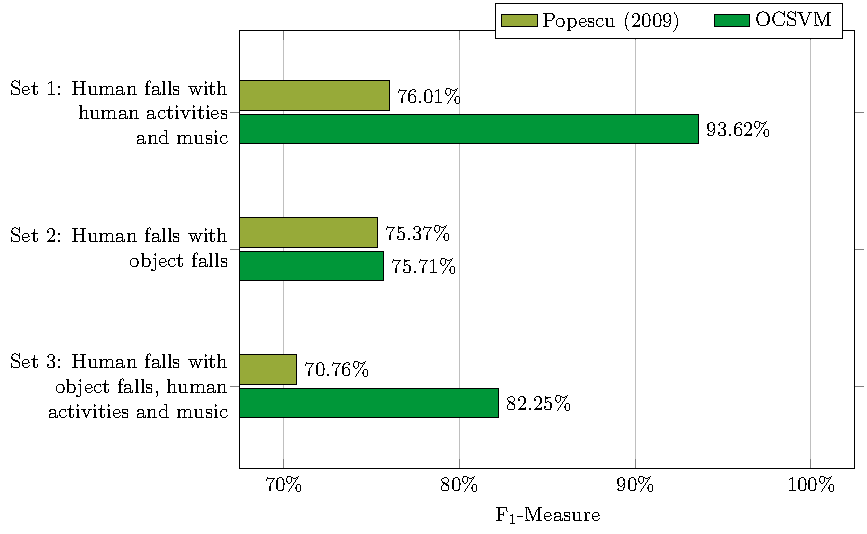
\includegraphics[width=\columnwidth]{img/cin_only_ocsv/res_clean.pdf}
	\caption{Results in \textit{clean} conditions for the three test cases. ``Set 1'' comprises human falls, human activities and music. ``Set 2'' comprises human falls and object falls. ``Set 3'' comprises human falls, object falls, human activities, and music.} \label{fig:res_clean}
\end{figure}

\figref{fig:res_noisy} shows the results obtained for the three cases in noisy conditions. As expected, the performance decreases in all the two evaluated methods. In ``Set 1'', the performance decrease is modest (2.32\% for the OCSVM and 1.44\% for ``Popescu (2009)''), demonstrating that the OCSVM is able to effectively reject non-fall events corrupted by music interference. In ``Set 2'', the presence object falls corrupted by music significantly decreases the performance of the OCSVM, reducing the F$_1$-Measure by 12.74\% with respect to the clean ``Set 2''. The method by Popescu and Mahnot \cite{Popescu2009} achieves the highest F$_1$-Measure in this case, confirming the good capabilities of rejecting dropping objects sound events observed in clean conditions. In ``Set 3'', the proposed approach improves the performance by 3.91\% with respect to ``Popescu (2009)'', confirming that it is able to achieve the highest performance in the most realistic scenario of the three.


\begin{figure}[t]
	\centering
	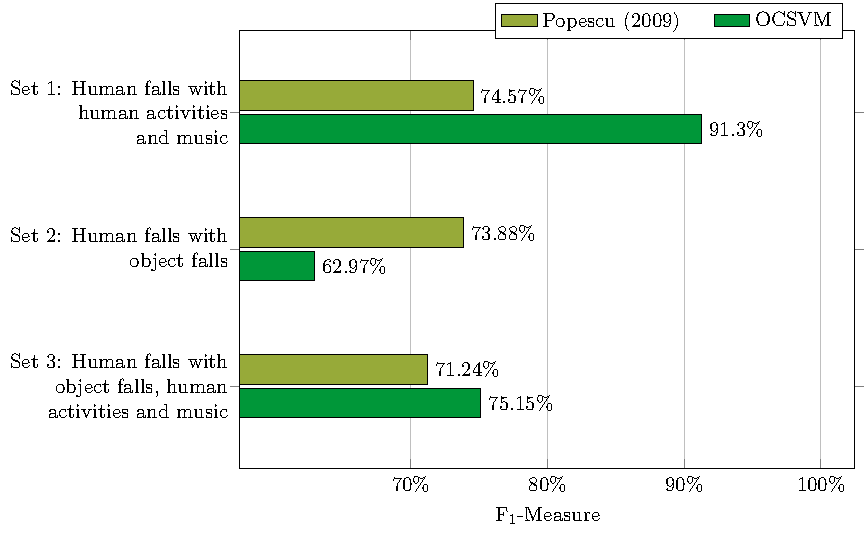
\includegraphics[width=\columnwidth]{img/cin_only_ocsv/res_noisy.pdf}
	\caption{Results in noisy conditions for the three test cases. ``Set 1'' comprises human falls, human activities and music. ``Set 2'' comprises human falls and object falls. ``Set 3'' comprises human falls, object falls, human activities, and music.} \label{fig:res_noisy}
\end{figure}




%\label{sec:ocsvm}}
\section{End-To-End Unsupervised Approach employing Convolutional Neural Network
Autoencoders for Human Fall Detection} 
\label{sec:autoencoder}



In recent years, thanks to the success of deep learning methods have become increasingly popular the feature learning approaches that independently transform the raw data inputs to a representation that can be exploited in machine learning tasks, minimizing the need of prior knowledge of application domain. 
Furthermore, such approaches are often able to generalize well real-world data compared to traditional hand-crafted features \cite{Principi14c}, resulting in an increase in performance of classification or regression tasks. The end-to-end learning is a particular example of feature learning, where the entire stack, connecting the input to the desired output, is learned from data \cite{muller2006off}. As in feature learning, only the tuning of the model hyperparameters requires some expertise, but even that process can be automated \cite{bergstra2013making}.

In this section, an end-to-end acoustic fall detection approach is presented. A deep convolutional neural network autoencoder is trained with the signals, gathered by the Floor Acoustic Sensor (\secref{sec:sensor}), corresponding to sounds that commonly occurring in a home (e.g., voices, footsteps, music, etc.). Since the sound produced by a human fall should be considerably different from the ones used for the training, it will be recognized as ``novelty'' by the network and classify as Fall. 
The performance of the algorithm has been evaluated on a subset of the dataset described in \secref{sec:dataset}, which contains human fall events simulated by employing the “Rescue Randy” human mimicking doll \cite{Werner2011,zigel2009method,alwan2006smart} and sounds related to common human activities.
Dieleman \textit{et al.} \cite{dieleman2014end} address the content-based music information retrieval tasks, investigating whether it is possible to apply end-to-end feature learning directly to raw audio signals instead that on a spectrogram representation of data.   
Up to the authors' knowledge, the end-to-end strategy has never been applied to a unsupervised fall detection approach with acoustic sensors. However, many works in other research fields can be founds in literature. 
Their convolutional neural networks trained on raw audio signals do not outperform a spectrogram-based approach in the automatic tagging task but are able to autonomously discover frequency decompositions from raw audio, as well as phase and translation-invariant feature representations.
The contribution is a novel fall detection method which exploits the end-to-end approach, resulting in a reduction of the engineering effort needed to design the system, with respect to those method that used features extracted from input signals. Is also shown that it can achieve good performance, higher than two state-of-the-art systems chosen for a comparison.


\section{Proposed Approach}
\label{sec:proposedApproach}

\begin{figure}[t]
	\centering
	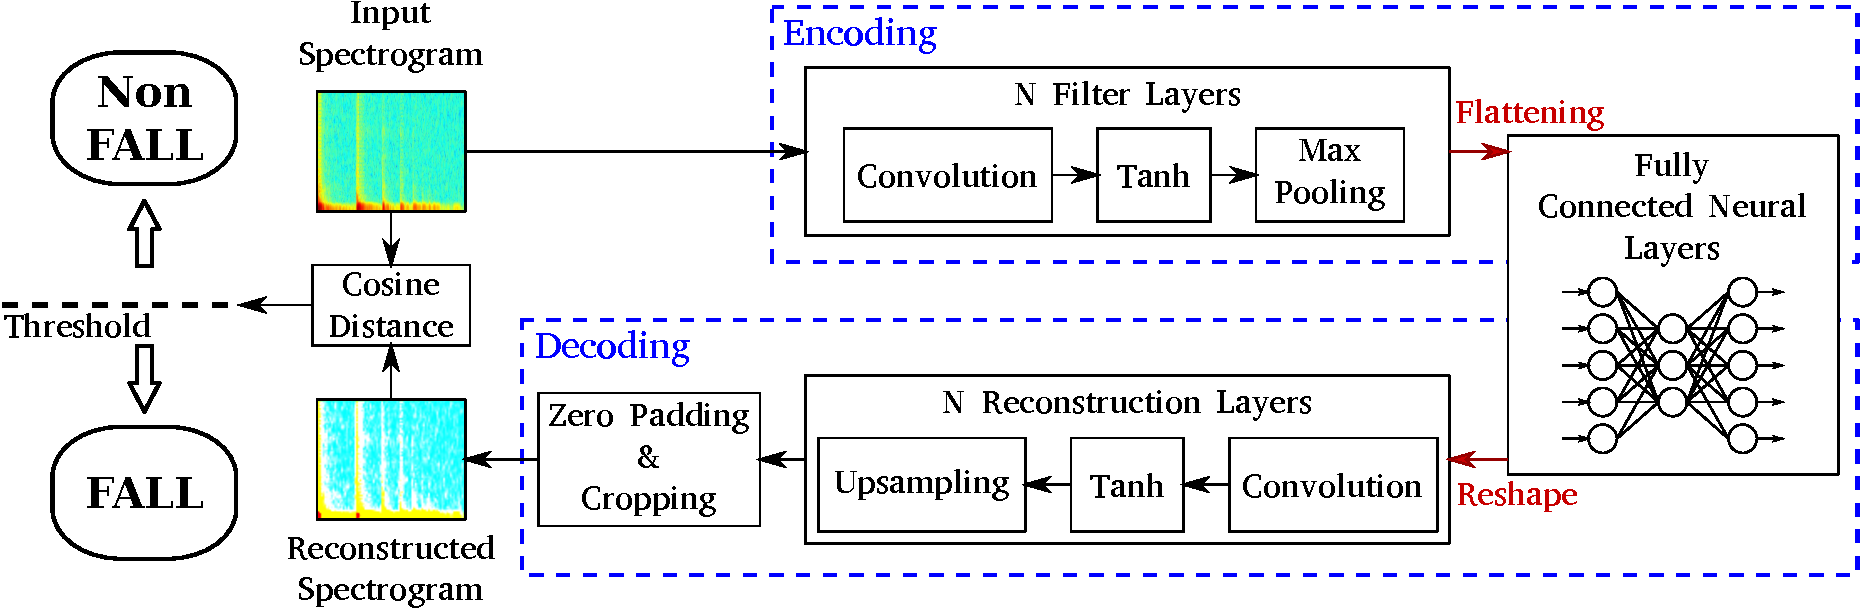
\includegraphics[width=\columnwidth]{img/wirn2017/approccioComplessivo.pdf}
	\caption{The proposed approach scheme.}\label{fig:overall}
\end{figure}

In the state of the art the majority of fall detection systems are logically designed as a cascade of elements which perform some sub-task (e.g. feature extraction, modeling, classification, ecc.).
%The minimal toolchain is composed by the feature extraction, modeling and classification blocks.
Each task is independently developed and generally requires the tuning of a number of hyperparameters using an experimental procedure and some a prior knowledge about the domain of the problem. 

The proposed approach, showed in \figref{fig:overall}, is designed according to the end-to-end paradigm and then, the entire stack, connecting the input to the desired output, is learned from data. 
End-to-End is a feature learning strategy that, in presence of sufficient training data, may result in better performance than systems based on handcrafted features, since the training procedure automatically select the salient information.
Therefore, if were possible to analyze the feature learned by the network with end-2-end strategy, there should be clues about what
kind of information is important for a specific task.

The system core is a deep convolutional neural network autoencoder. Some exhaustive discussion about this type of network can be easily  found in literature \cite{ng2011sparse,krizhevsky2012imagenet,marchi2017deep}. 
The network input consists of the normalized log-power spectrograms of the signals calculated with a STFT on windows of 32 ms and overlapped by 50\%.
Due to the presence of fully-connect neural layers, the input dimensions must be fixed. After having identified the widest spectrogram extracted from the dataset, the other ones have been extended with some AWGN frames added at the end. Each input consist in a $f\times t$ matrix, where $f$ are the positive points of discrete Fourier transform and $t$ are the number of windows considered in time.
The output of the autoencoder are the reconstructed spectrograms. To classify an event, a distance measurement between input and output must be made with some heuristic. If the distance exceeds a certain threshold, automatically defined by the algorithm during the training phase, the system label the output as "Fall" or as "Non Fall" otherwise. In this work the cosine distance has been used:

%f=129 t=197

\begin{equation}
D_C(v,u)=1-\frac{u\cdot v}{\left\|u \right\|\left\|v \right\| }= 1- \frac{\sum_{k=1}^{n}u(k)v(k)}{\sqrt{\sum_{k=1}^{n}u(k)^2}\sqrt{\sum_{k=1}^{n}v(k)^2}}
\end{equation}
where $u$ and $v$ are the the vectors obtained flattening the input and the output spectrograms and $n$ are the length of this vectors. 
According to the cosine definition, the value of the distance always has a value between $-1$ and $+1$, where $+1$ indicates two equal vectors while $-1$ indicates two opposite vectors.
The added AWGN part of the spectrums was not considered to calculate the distance. The choice of this heuristic allowed to make distance measurements independents of the size of the initial spectrum.
The structure of the autoencoder is not defined a priori, but it is chosen through a phase of cross-validation during which the network parameters are varied with a random search strategy.

\section{Experiments}
\label{sec:endtoend_experiments}
In this section are described the composition of the dataset used in this work and the experimental set-up.

\subsection{Dataset} 

The instances used in this approach are summarized in table \tableref{tab:endtoend_dataset}.
It is composed of two type of sounds: the first, namely novelty, comprises several human fall sounds that have been simulated by means of a human-mimicking doll employed in water rescues. The doll has been dropped from upright position and from a chair, both forward and backward. The drops have been then repeated at three distances from the FAS, i.e., 2, 4 and 6 m, for a total of 44 events, all included in the “Human fall” class. The second type, i.e, the background, comprises sounds of normal activities (voices, footsteps, etc.) for a total of 1218 s, and three musical tracks\footnote{W. A. Mozart, ``Piano trio in C major''}\footnote{Led Zeppelin, ``Dazed and confused''}\footnote{Led Zeppelin, ``When the levee breaks''}, for a total of 1498 s, played from a loudspeaker and acquired back with the FAS.
In addition, the signals of the second type have been employed alone and to create noisy versions of human falls occurrences in order to assess the algorithm in presence of interferences.
The signals have been acquired with a sampling rate equal to 44.1 kHz and 32 bit depth. Based on previous experience in using the FAS, in order to exploit the acoustic characteristics of the sensor, signals have been downsampled to 8 kHz and the resolution has been reduced to 16 bit.


\begin{table}[t]
	\caption{Composition  of the dataset.}
	\label{tab:endtoend_dataset}
	\begin{center}
		\begin{tabular}[t]{c>{\centering}m{5cm}c}
			
			\hline
			\textbf{Class} & \textbf{Nr. of occurrences} & \textbf{Total length (s)} \\ %\cline{2-5} 
			%& \hspace{8pt}Clean\hspace{8pt}  & \hspace{6pt}Clean\hspace{6pt}   \\ 
			\hline

			$\,$ Human Falls $\,$ 	& 44    &   76     \\
			Human Activity  		& 665   &   1218     \\
			Music					& 776   &	1498	\\
			%				 Classic Music       	& 441   &   882     \\
			%				 Rock Music       		& 335   &   616     \\
			\hline
		\end{tabular}
	\end{center}
\end{table}

\subsection{Experimental Setup}

Since in this work a novelty approach is presented, the dataset has been divided in two groups: the former composed only of background sounds (i.e human activity sounds and musical background) used for the training; the latter composed of both background sound and novelty sounds, i.e, the human falls, used in development and test phase.
In order to assess the classification accuracy in noisy conditions, a second version of human fall sounds were crated in which a musical background was recorded and then digitally added to the fall events.

The input spectrograms of the audio signals has been calculated with a fft point number of 256 and a windows size of 256 samples (32 ms at sample rate of 8000 kHz). The longest spectrogram present in the dataset is composed of 197 frame. Therefore the resulting input matrix  dimension $f\times t$ is $129\times 197$.
The optimization of the experiment hyper-parameters has been carried out using the random-search technique. \tableref{tbl:hyper-params} shows the parameters used in the random-search, and their ranges. The parameters of the network architecture are related only to the encoding part of autoencoder since the decoding part is its mirrored version. 
Instead other parameters, described below, have been set to the same value for all experiments. The activation function for each layer, whether they are convolutional or fully connected, have been set to $tanh$. ``Adam'' \cite{kingma2014adam} has been used as optimization algorithm for the traing phase. The loss function used was $mlse$. The initialization algorithm for the weight of the autoencoder was Glorot Uniform \cite{glorot2010understanding}. The number of epoch has been set to 1000, while the patience, that is the number of epoch without an Auc improvement on a devset to wait before stopping the training phase, has been set to 40.

In order to implements a 4 fold cross-validation, the signals not being part of training-set have been divided in four folds, each composed of 11 human falls and 11 non-falls signals. Then, one fold has been used as validation-set and the remaining three for calculating the performance in test phase. In cross-validation phase the scores have been evaluated in term of AUC. Here also the optimal thresholds have been infer by searching points on ROC curves closest to the $(0, 1)$: $ d_{min} = \sqrt{(1-fpr)^{2}+(1-tpr)^{2}} $.
At the end the final performance has been evaluated in term of  $ F_1 -Measure$ by mediating the results obtained on individual folds.

\begin{table}[t]
	\caption{Hyper-parameters optimized in the random-search phase, and their range.}\label{tbl:hyper-params}
	\centering
	\footnotesize
	\begin{tabular} {|c | c | c|| c | c | c|}
		\hline
		Parameter 		& Range & Distribution &Parameter & Range & Distribution\\  
		\hline\hline
		Cnn layer Nr. 	& [1-3]& uniform & Batch size	&	[10\%-25\%] & log-uniform\\
		\hline
		Kernel shape 	& [3x3-8x8]& uniform & Max pool shape & [1x1-5x5] & uniform \\
		\hline									
		Kernel Nr. 		& [4-64]& log-uniform & Max Pool & All\tablefootnote{After each Conv. layer}-Only end\tablefootnote{At the end of cnn part}& uniform \\
		\hline                                     
		MLP layers Nr. 	&	[1-3]& uniform & Dropout & [Yes-No] & uniform\\% dense-layer da uno a tre perchè quello interno ci sta sempre + da 0 a 2 di quelli messi dopo 
		\hline
		MLP layers dim.	&	[128-4096]& log-unifom & Drop rate	&	[0.5-0.6] & normal\\
		\hline
		Stride & [1x1-3x3]& uniform & Learning rate	&	[$10^{-4}$-$10^{-2}$]  & log-unifom\\
		\hline
		
	\end{tabular}
\end{table}
Since this approach share the same train-set (\tableref{tab:trainComposition}) and test-set (\secref{tab:set1Composition}) that has been used in \secref{sec:ocsvm_approach} for both the clean and noisy conditions, the results scored here were compared with those obtained showed in \figref{fig:res_clean} and related to Set 1.

\begin{table}[t]
	\caption{Best hyper-parameters find in random-search phase for \textit{clean} and \textit{noisy} condition}\label{tbl:best-clean-params}
	\centering
	\footnotesize
	\resizebox{\textwidth}{!}{	\begin{tabular} {|c |  c | c | c | c ||  c | c | c | c |}
			\hline
			&\multicolumn{4}{|c||}{Clean}&\multicolumn{4}{c|}{Noisy}\\
			\hline
			Parameter		& Fold1 &Fold2 &Fold3 & Fold4  & Fold1 & Fold2 & Fold3 & Fold4\\
			\hline
			Cnn layer Nr.	& 3 & 3 & 3 & 2 & 3 & 3 & 3 & 3\\
			\hline
			Kernel shape 	& 8x8 & 7x7 & 5x5 & 8x8 & 8x8 & 7x7 & 8x8 & 8x8 \\
			\hline
			Kernel Nr. 	& [16,16,8] & [32,16,16] & [8,8,8]& [32,16] & [32,32,8] &  [32,32,8] &  [32,32,32] & [8,8,8]\\
			\hline
			Max Pool Position		&only end &only end & all& all & only end & only end & all & only end\\
			\hline
			Max pool shape	& 5x5 & 3x3 & 5x5 & 4x4 & 3x3 & 5x5 & 5x5 & 3x3\\
			\hline
			Stride	& 3x3 & 3x3 & 1x1 & 3x3 & 3x3 & 3x3 & 1x1 & 3x3\\
			\hline
			MLP layers Nr. & 2 & 1 & 1 & 1 & 2 & 2 & 1 & 3\\
			\hline
			MLP layers dim.	& [16,231] & 96 & 32 & 32  & [48,153] & [16,2084] & 128 & [48,1952,1952]\\
			\hline
			%Learning rate	&$\num{4.89e-4}$ &  $\num{0.408e-4}$ & $\num{1.509e-4}$ &  $\num{1.544e-4}$ & $\num{0.156e-4}$ &  $\num{0.446e-4}$ & $\num{0.101e-4}$ &  $\num{0.100e-4}$\\
			Learning rate$(\times\num{e-4})$&4.89 &  4.08 & 15.09 &  15.44 & 1.56 &  4.46 & 1.01 &  1.00\\
			\hline
			Batch size		& 11.26\% & 10.81\% & 13.59\% & 21.10\% & 20.06\% & 12.55\% & 13.51\% & 13.13\%  \\
			\hline
			Drop rate		&0.64 &0.57 & 0.53 & 0.55  & 0.58 &0.53 & 0.55 & 0.59\\	
			\hline	
			
	\end{tabular}}
\end{table}

\subsection{Results}
The results for both clean and noisy are reported in \figref{fig:endtoend_results}. The comparative algorithms are denoted with ``Popescu (2009)'' and ``OCSVM'' respectively, while the proposed approach is named ``Autoencoder''. It is immediately clear that the proposed approach outperforms the other in both conditions. In fact, in clean condition, it gains about 1\% compared to ``OCSVM'' and about 18.6\% compared to ``Popescu (2009)''. Moreover the proposed algorithm results to be very robust in noisy condition, %where the score of ``OCSVM'' falls down %by 30.65\% while the score of  ``Popescu (2009)'' remains around the previous case.
whereas both other cases get worse a bit.
In particular the performance improves by 3.72\% with respect to ``OCSVM'' and by 20.45\% with respect to ``Popescu (2009)''. Clearly the end-to-end method seems insensitive with respect to the corrupted human fall signals when the novelty sounds are dissimilar respect to normality model learned from the background sounds. 
In \tableref{tbl:best-clean-params} are reported the hyperparameters that have led to the results discussed above.

Furthermore other experiments were made up with a manual tuning of parameters. Particularly have been investigated deeper architectures composed up to 5 convolutional layer. We found that increasing the depth on cnn part (5 layers) with a different kernel number for each layers of [32,32,16,16,8] and a kernel dimension for all layers of 4x4, a max pooling after only the first three convolutional layer of 2x2 and two MLP layer of 1024 and 512, leads to considerable improvements. In effect the final $ F_1 -Measure$ rise up to 95,42\%  in both clean and noisy condition. 
%\textcolor{red}{per motivare che noisy is better than clean direi che è dovuto allla variabilità degli esperimenti (inizializzazioni varie ecc..) visto che cmq c'è lo scarto di un solo mezzo punto. Se ripetessimo gli esperimenti potremmo ottenere risultati leggermente diversi ( considerando anche che siamo anche in cross-validation) }


\begin{figure}[t]
	\centering
	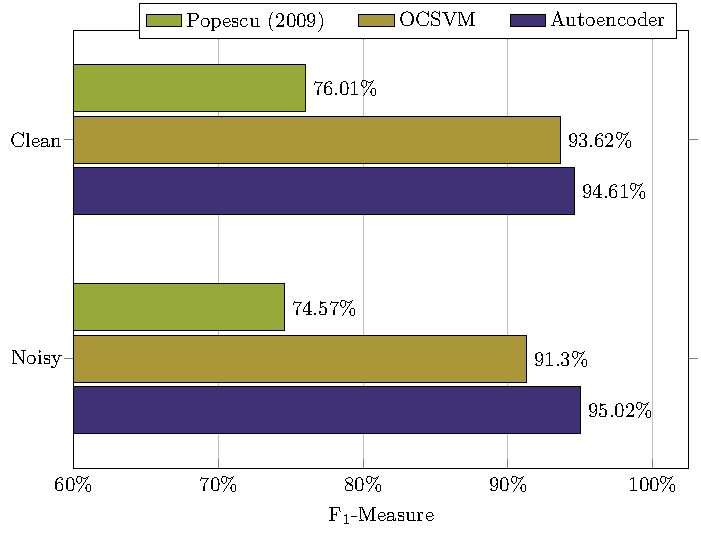
\includegraphics[width=0.75\columnwidth]{img/wirn2017/grafTex/results.pdf}
	\caption{Results in \textit{clean} and \textit{noisy} conditions for the three test cases.} 
	\label{fig:endtoend_results}
\end{figure}

\subsection{Remarks}
The methods presented is an end-to-end approach composed by a deep-convolutional-autoencoder with a downstream threshold classifier, that is a purely unsupervised approach to acoustic fall detection.
Our method exploits the reconstruction error of the autoencoder. When a sound that the network has never seen in training phase occurs, the reconstruction error raise up allowing the recognition of novelty.
The algorithm has been trained with a large corpus of background signals, i.e, human activity noise and music, and evaluated with human-fall sound and other instances of background sounds. It has been evaluated in two different condition: the first with a clean version of human fall sounds and the second with corrupted version of the same.
The results showed that the proposed solution leads to an average improvement about 20\%  with respect to the \cite{Popescu2009} and about 2.3\% towards the OCSVM based approach.

In future works this approach will be assessed in a more realistic scenario including, in the test phase, others sound topologies such as falls of different objects, street sounds, etc., that could compromise the classification. In fact those sounds are much more similar to the human falls and could lead to a worse performance. In addition, having regard the results obtained with a manual tuning of parameters, deeper network architectures in combination with Recurrent Neural Network will be thoroughly investigated.

